
In this chapter we give a brief summary of Erlang and RefactorErl tool.

\section{An introductory glimpse at the Erlang programming language}
Erlang is a functional language and accompanying runtime designed for highly
parallel, scalable applications requiring high uptime. Erlang is a programming
language designed for developing robust systems of programs that can be distributed among different computers in a network.Erlang is similar to Java in that it uses a virtual machine and supports multithreading. 

\textbf{Variables}
Erlang provides dynamic data types, allowing programmers to develop system
components (such as message dispatchers) that do not care what type of data they are handling and others that strongly enforce data type restrictions or that decide how to act based on the type of data they receive.Variables must begin with a capital letter or an underscore, and are composed of letters, digits, and underscores.

\textbf{Data types}
Erlang has:
\begin{enumerate}
	\item Integers, of unlimited size.
	\item Floats.
	\item Strings, enclosed in double quotes: "This is a string.".
	\item Atoms. An atom stands for itself. It begins with a lowercase letter and is composed of letters, digits, and underscores, or it is any string enclosed in single quotes: atom1, 'Atom 2'.
	\item Lists, which are a comma-separated sequence of values enclosed in brackets: [abc, 123,"pigs in a tree"]. 
	\item Tuples, which are a comma-separated sequence of values enclosed in braces: {abc, 123,"pigs in a tree"}.
	\item Records, which are not a separate data type, but are just tuples with keys associated with each value. They are declared in a file and defined (given specific values) in the program.
	\item Binaries, enclosed in double angle brackets: <<0, 255, 128, 128>>, <<"hello">>, <<X:3,Y:7, Z:6>>. Binaries are sequences of bits; the number of bits in a binary must be a multiple of 8.
	\item References are globally unique values.
	\item Process identifiers (Pids) are the "names" of processes.
\end{enumerate}

Figure \ref{fig:example_erlang}features the source of a small Erlang program
called example that demonstrated recursive list manipulation.
\begin{figure}[h]
	\begin{lstlisting}[extendedchars=true, language=Erlang, basicstyle=\footnotesize\ttfamily, keywordstyle=\color{red}]
	-module(example). 
	-export([max/1, min/1, sum/1]).
	
	%% Find the maximum of a list.
	max([H|T]) -> max2(T, H).
	max2([], Max) -> Max;
	max2([H|T], Max) when H > Max -> max2(T, H);
	max2([_|T], Max) -> max2(T, Max).
	

	%% Find the minimum of a list.
	min([H|T]) -> min2(T,H).
	min2([], Min) -> Min;
	min2([H|T], Min) when H < Min -> min2(T,H);
	min2([_|T], Min) -> min2(T, Min).
	
	%% Find the sum of all the elements of a list.
	sum(L) -> sum(L,0).
	sum([], Sum) -> Sum;
	sum([H|T], Sum) -> sum(T, H+Sum).
	\end{lstlisting}
\caption{A simple module in Erlang.}
\label{fig:example_erlang}
\end{figure}

Erlang source files consist of a section containing meta-information about the module represented by the file(all functions in Erlang must be defined in
modules.), and a list of functions that are either exposed to the users of this module (with the -export attribute), or are only defined for internal use inside the module.  

A subtle element of all three functions is that every function needs to 
have an initial value to start counting with. In the case of 
sum/2, we use 0, as we’re doing addition, and given X = X + 0, the value is neutral, so we can’t mess up the calculation by starting there. If we were doing multiplication, we would use 1 given X = X * 1. 

The functions min/1 and max/1 can’t have a default starting value. If the 
list were only negative numbers and we started at 0, the answer would be 
wrong. So we need to use the first element of the list as a starting point.

\section{The RefactorErl static analysis framework} 

RefactorErl~\cite{refactorerl1, refactorerl2} is an open-source static source code analyzer and transformer tool for Erlang,developed by the Department of Programming Languages and Compilers at the Faculty of Informatics, Eötvös Loránd University, Budapest, Hungary. The phrase "refactoring" means a preserving source code transformation, so while you change the programstructure you do not alter its behaviour. RefactorErl was built to refactor Erlang programs.

The main focus of RefactorErl is to support daily code comprehension tasks of Erlang developers. It can analyse the structure of the refactored program - based on the syntactic rules of the underlying programming language - and it can also collect and use semantical information about the source code.

\subsection{Metrics in the RefactorErl}

A metric query language is incorporated into RefactorErl~\cite{refactorerl} . Metric queries can be executed from the console interface or can be used as properties in semantic query language which is available from every interface.

Table \ref{tab:metrics_ref} shows all the implemented metrics in RefactorErl tool. There are two coloms in this table: the first column gives the information about the name of the metric, and the second column shows the for which node the metric is available.

\begin{table}[!htb]
	\centering
	\caption{Implemented metrics in RefactorErl}
	\label{tab:metrics_ref}
	\noindent\adjustbox{max width=0.9\textwidth}{
		\begin{tabular}{|c|c|}
			\hline
			\textbf{Name of the metric}  & \textbf{Node type} 
			\\
			\hline
			module sum					& module
			\\
			
			\hline
			line of code				& module/function
			\\
			
			\hline
			char of code				& module/function
			\\
			
			\hline
			number of fun				& module
			\\
			
			\hline
			number of macros			& module
			\\
			
			\hline
			number of records			& module
			\\
			
		  	\hline
			included files				& module
			\\	
				
		  	\hline
		  	imported modules			& module
		  	\\	
		  	
		  	\hline	
		  	number of funpath			& module
		  	\\	

		  	\hline
		  	function calls in			& module
		  	\\
		  	
		  	\hline
		  	function calls out			& module
		  	\\	
		  	
		  	\hline
		  	cohesion					& module
		  	\\	  	
		  	
		  	\hline
		  	function sum				& function
		  	\\	  	
		  			  	
		  	\hline
		  	max depth of calling		& module/function		  			  
		  	\\
		  	
		  	\hline
		  	max depth of cases			& module/function		  			  
		  	\\		
		  	  	
		  	\hline
		  	min depth of cases			& module/function		  			  
		  	\\		  	

		  	\hline
		  	max depth of structs		& module/function		  			  
		  	\\		  			

		  	\hline
		  	number of funclauses		& module/function		  			  
		  	\\			
	
		  	\hline
		  	branches of recursion		& module/function		  			  
		  	\\			

		  	\hline
		  	calls for function			& function		  			  
		  	\\			
			
		  	\hline
		  	calls from function			& function		  			  
		  	\\	

		  	\hline
		  	number of funexpr			& module/function		  			  
		  	\\
		  	
		  	\hline
		  	number of messpass			& module/function		  			  
		  	\\		  	

		  	\hline
		  	fun return points			& module/function		  			  
		  	\\	
		  	
		  	\hline
		  	average size				& module/function		  			  
		  	\\		  		  	

		  	\hline
		  	max length of line			& module/function		  			  
		  	\\
		  	
		  	\hline
		  	no space afte  comma		& module/function		  			  
		  	\\	
		  	
		  	\hline
		  	is tail recursive			& function		  			  
		  	\\		  	

		  	\hline
		  	mcCabe						& module/function		  			  
		  	\\	
		  			  	
		  	\hline
		  	otpused						& module		  			  
		  	\\			  	
		  	\hline		  		  			  				
		\end{tabular}}
	\end{table}

\textbf{module\_sum}

The domain of the query is a module. The sum of the chosen complexity structure metrics measured on the modules functions. The proper metrics adjusted in a list can be implemented in the desired number and order~\cite{refactorerl}.

\textbf{line\_of\_code}

The domain of the query is a module or a function. The number of the lines of part of the text, function, or module. The number of empty lines is not included in the sum. As the number of lines can be measured on more functions, or modules and the system is capable of returning the sum of these, the number of lines of the whole loaded program text can be enquired~\cite{refactorerl}.

\textbf{char\_of\_code}

The domain of the query is a module or a function. The number of characters in a program script. This metric is capable of measuring both the codes of functions and modules and with the help of aggregating functions we can enquire the total and average number of characters in a cluster, or in the whole source text~\cite{refactorerl}.

\textbf{number\_of\_fun}

The domain of the query is a module. This metric gives the number of functions
implemented in the concrete module, but it does not contain the number of non-defined functions in the module~\cite{refactorerl}.

\textbf{number\_of\_macros}

The domain of the query is a module. This metric gives the number of defined macros in the concrete module, or modules. It is also possible to enquire the number of implemented macros in a module~\cite{refactorerl}.

\textbf{number\_of\_records}

The domain of the query is a module. This metric gives the number of defined records in a module. It is also possible to enquire the number of implemented records in a module~\cite{refactorerl}.

\textbf{included\_files}

The domain of the query is a module. This metric gives the number of visible header files in a module~\cite{refactorerl}.

\textbf{imported\_modules}

The domain of the query is a module. This metric gives the number of imported modules used in a concrete module. The metric does not contain the number of qualified calls (calls that have the following form: module:function)~\cite{refactorerl}.

\textbf{number\_of\_funpath}

The domain of the query is a module. The total number of function paths in a module.The metric, besides the number of internal function links, also contains the number of external paths, or the number of paths that lead outward from the module. It is very similar to the metric called cohesion~\cite{refactorerl}.

\textbf{function\_calls\_in}

The domain of the query is a module. Gives the number of function calls into a module from other modules. It can not be implemented to measure a concrete function. For that we use the calls\_for/1 function~\cite{refactorerl}.

\textbf{function\_calls\_out}

The domain of the query is a module. Gives the number of every function call from a module towards other modules. It can not be implemented to measure a concrete function. For that we use the calls\_from/1 function~\cite{refactorerl}.

\textbf{cohesion}

The domain of the query is a module. The number of call-paths of functions that call eachother. By call-path we mean that an f1 function calls f2 (e.g. f1()->f2().). If f2 also calls f1, then the two calls still count as one call-path~\cite{refactorerl}.

\textbf{function\_sum}

The domain of the query is a function. The sum calculated from the functions complexity metrics that characterizes the complexity of the function. It can be calculated using various metrics together~\cite{refactorerl}.
	 
\textbf{max\_depth\_of\_calling}

The domain of the query is a module or a function. The length of function call-chains, namely the chain with the maximum depth~\cite{refactorerl}.
	 
\textbf{max\_depth\_of\_cases}

The domain of the query is a module or a function. Gives the maximum of case control structures embedded in case of a concrete function (how deeply are the case control structures embedded). In case of a module it measures the same regarding all the functions in the module. Measuring does not break in case of case expressions, namely when the case is not embedd~\cite{refactorerl}.

\textbf{min\_depth\_of\_cases}

The domain of the query is a module or a function. Gives the minimum of the maximums of case control structures embedded in case of a concrete function (how deeply are the case control structures embedded). In case of a module it measures the same regarding all the functions in the module. Measuring does not break in case of case expressions, namely when the case is not embedded into a case structure. However, the following embedding does not increase the sum~\cite{refactorerl}.

\textbf{max\_depth\_of\_structs}

The domain of the query is a module or a function. Gives the maximum of structures embedded in function (how deeply are the block, case, fun, if, receive, try control structures embedded). In case of a module it measures the same regarding all the functions in the module~\cite{refactorerl}.

\textbf{number\_of\_funclauses}

The domain of the query is a module or a function. Gives the number of a functions clauses. Counts all distinct branches, but does not add the functions having the same name, but different arity, to the sum~\cite{refactorerl}.

\textbf{branches\_of\_recursion}

The domain of the query is a module or a function. Gives the number of a certain function's branches, how many times a function calls itself, and not the number of clauses it has besides definition~\cite{refactorerl}.

\textbf{calls\_for\_function}

The domain of the query is a function. This metric gives the number of calls for a concrete function. It is not equivalent with the number of other functions calling the function, because all of these other functions can refer to the measured one more than once~\cite{refactorerl}.

\textbf{calls\_from\_function}

The domain of the query is a function. This metric gives the number of calls from a certain function, namely how many times does a function refer to another one (the result includes recursive calls as well)~\cite{refactorerl}.

\textbf{number\_of\_funexpr}

The domain of the query is a module or a function. Gives the number of function expressions in a module. It does not measure the call of function expressions, only their initiation~\cite{refactorerl}.

\textbf{number\_of\_messpass}

The domain of the query is a module or a function. In case of functions it measures the number of code snippets implementing messages from a function, while in case of modules it measures the total number of messages in all of the modules functions~\cite{refactorerl}.

\textbf{fun\_return\_points}

The domain of the query is a module or a function. The metric gives the number of the functions possible return points (or the functions of the given module)~\cite{refactorerl}.

\textbf{average\_size}

The domain of the query is a module or a function. The average value of the given complexity metrics (e.g. Average branches\_of\_recursion calculated from the functions of the given module)~\cite{refactorerl}.

\textbf{max\_length\_of\_line}

The domain of the query is a module or a function. It gives the length of the longest line of the given module or function~\cite{refactorerl}.

\textbf{average\_length\_of\_line}

The domain of the query is a module or a function. It gives the average length of the lines within the given module or function~\cite{refactorerl}.

\textbf{no\_space\_afte\r\_comma}

The domain of the query is a module or a function. It gives the number of cases when there are not any whitespaces after a comma or a semicolon in the given module's or function's text~\cite{refactorerl}.

\textbf{is\_tail\_recursive}

The domain of the query is a function. It returns with 1, if the given function is tail recursive; with 0, if it is recursive, but not tail recursive; and -1 if it is not a recursive function (direct and indirect recursions are also examined). If we use this metric from the
semanctic query language, the result is converted to tail\_rec, non\_tail\_rec or non\_rec atom~\cite{refactorerl}.

\textbf{mcCabe}

McCabe cyclomatic complexity metric. Available for modules and functions. We define it based on the control flow graph of the functions with the number of different execution paths of a function, namely the number of different outputs of the function~\cite{refactorerl}.

\textbf{otp\_used}

Gives the number of OTP callback modules used in modules~\cite{refactorerl}.

\section{Metric visualisation module for WEB2 interface of RefactorErl}

The section describes the main concept and details of the developed module for RefactorErl static analyzis tool.

\subsection{Description of the software}

The program allows to analyze git repositories with Erlang code. The main feautures are:
\begin{itemize}
	\item Drawing plots which show change of metrics with software evolving from version to version.
	\item Analyzing modules and functions separately.
	\item Choosing separate files for the analyzing.
	\item User-friendly web interface.
\end{itemize}

The main focus of the project is to help Erlang developers with analyzing their projects using plots. Visualisation helps with finding patterns and improving of code quality. 

\subsection{Used tools}

\textbf{NVD3}

Inspired by Mike Bostock and currently maintained by a team of frontend software engineers at Novus Partners, NVD3 is another quality D3 based JavaScript library.Allowing you to create beautiful reusable charts in your web applications.

It has great features for visualizing data with lovely charts such as the box-plot, sunburst and candlestick charts. If you are looking for tons of functionality in a JavaScript charting library, NVD3 is the one to look out for.

\textbf{AngularJs}

The new component was created for existing system using this javascript web framework.

AngularJS (also written as Angular.js) is a JavaScript-based open-source front-end web application framework mainly maintained by Google and by a community of individuals and corporations to address many of the challenges encountered in developing single-page applications.

The AngularJS framework works by first reading the Hypertext Markup Language (HTML) page, which has additional custom tag attributes embedded into it. Angular interprets those attributes as directives to bind input or output parts of the page to a model that is represented by standard JavaScript variables. The values of those JavaScript variables can be manually set within the code, or retrieved from static or dynamic JSON resources. 

\textbf{DETS tables}

Data of calculated metrics for modules and functions stored in two different tables: mods\_metrics and funs\_metrics.

DETS is Disk Erlang Term Storage. DETS tables store tuples, with access to the elements given through a  key field in the tuple. The tables are implemented using hash tables and binary trees, with different representations providing different kinds of collections~\cite{erland_o'reilly}.

\textbf{JSON}

Data which stored in Dets tables transforms into JSON objects when Erlang code interact with JavaScript code.
JSON (JavaScript Object Notation) is a lightweight data-interchange format.
JSON is a text format that is completely language independent but uses conventions that are familiar to programmers of the C-family of languages, including C, C++, C\#, Java, JavaScript, Perl, Python, and many others. These properties make JSON an ideal data-interchange language.

JSON is built on two structures:
\begin{itemize}
	\item A collection of name/value pairs. In various languages, this is realized as an object, record, struct, dictionary, hash table, keyed list, or associative array.
	\item An ordered list of values. In most languages, this is realized as an array, vector, list, or sequence.
\end{itemize}

\subsection{The typical workflow}

For using the component WEB2 interface should be run. It can be done with this command executed in RefactorErl shell:

\begin{lstlisting}[frame=none, numbers=none]
	ri:start_web2([{yaws_path, PATH-TO-YAWS}]).
\end{lstlisting}

This command will run WEB2 interface available on localhost:8001 by default. After loginning the component can be accessed in metrics tab as shown on Figure \ref{fig:metrics_interface}

\begin{figure}[h]
	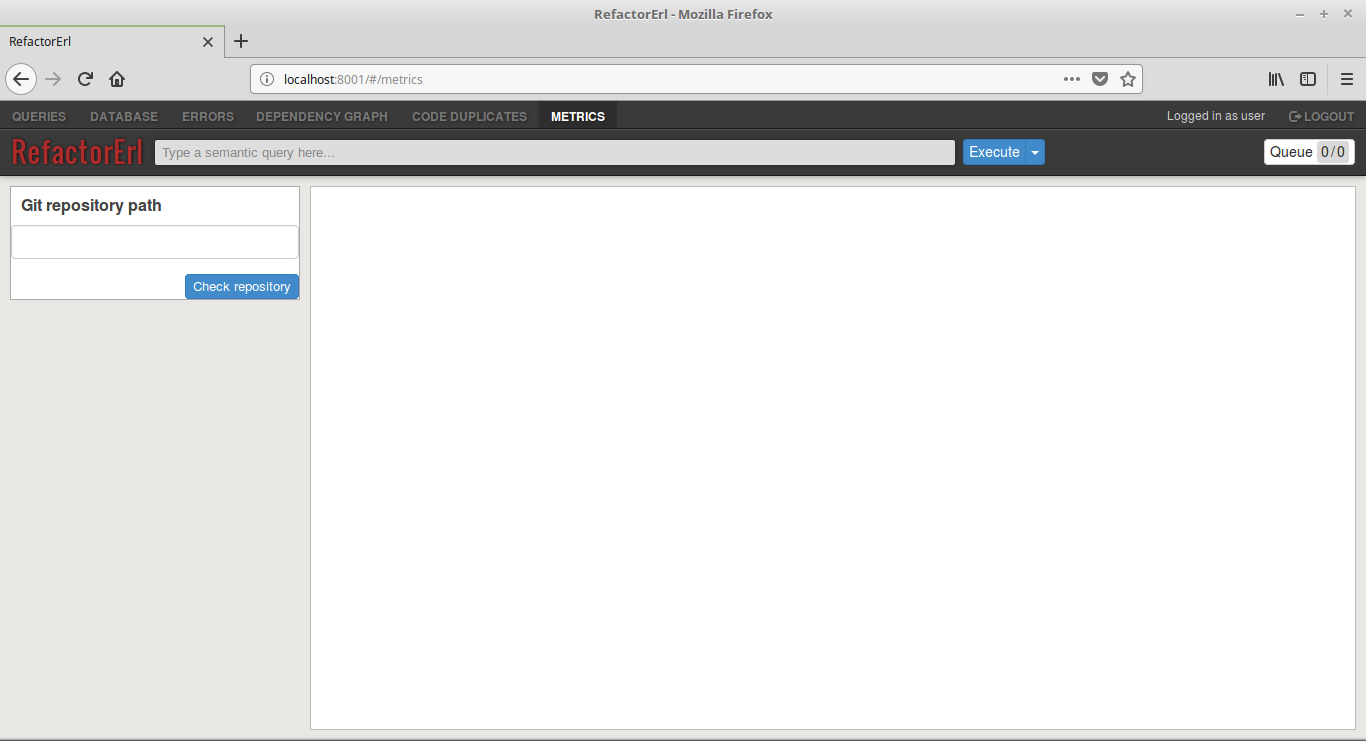
\includegraphics[height=80mm]{figures/metrics.png}
	\caption{Component interface.}
	\label{fig:metrics_interface}
\end{figure}

The path to git repository should be provided in "Git repository path" input. After clicking the "Check repository" button the folder will be analized. If it is not valid the alert Figure \ref{fig:metrics_alert} will be shown.  

\begin{figure}[h]
	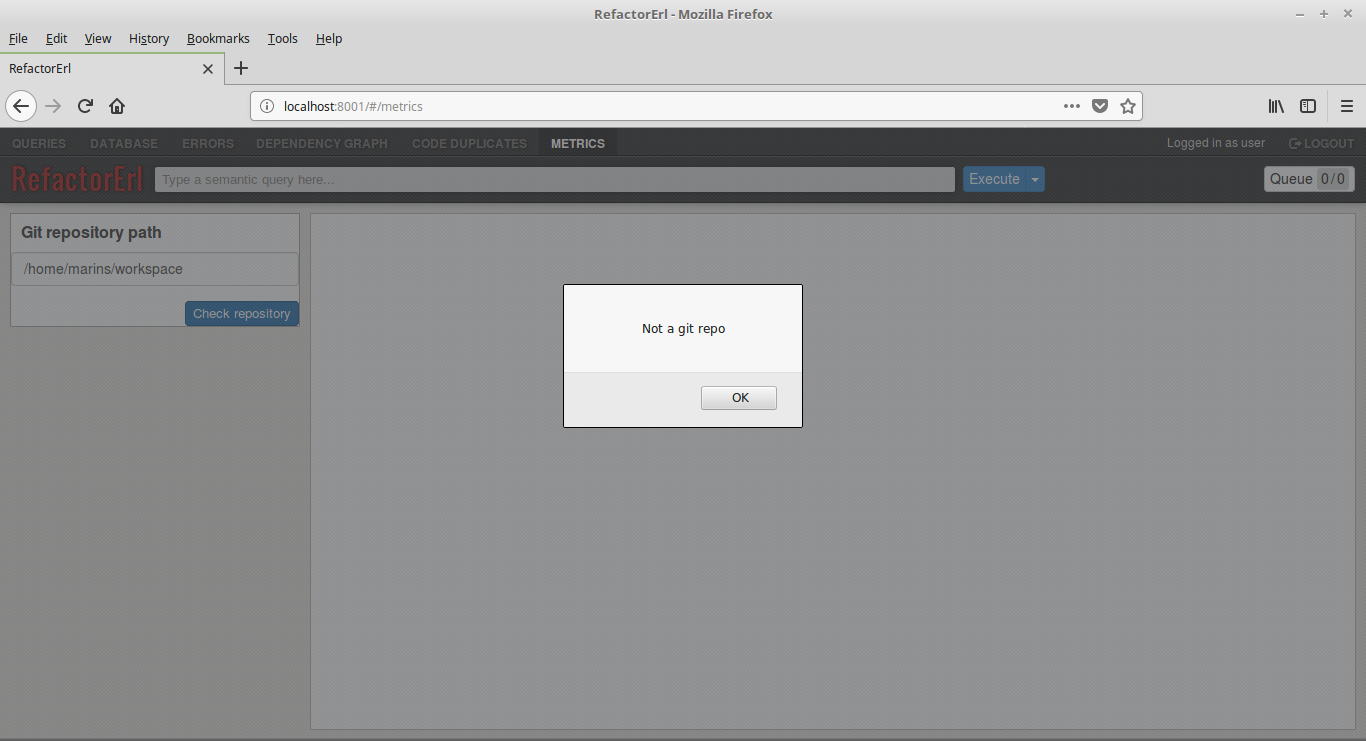
\includegraphics[height=80mm]{figures/alert.png}
	\caption{Alert shown because the provided folder is not a valid repository.}
	\label{fig:metrics_alert}
\end{figure}

In other case the folder tree will be available where separate files can be choosen for future analyzing as shown at Figure \ref{fig:metrics_files}. Also there is a possibility to delete some files choosen by mistake.

\begin{figure}[h]
	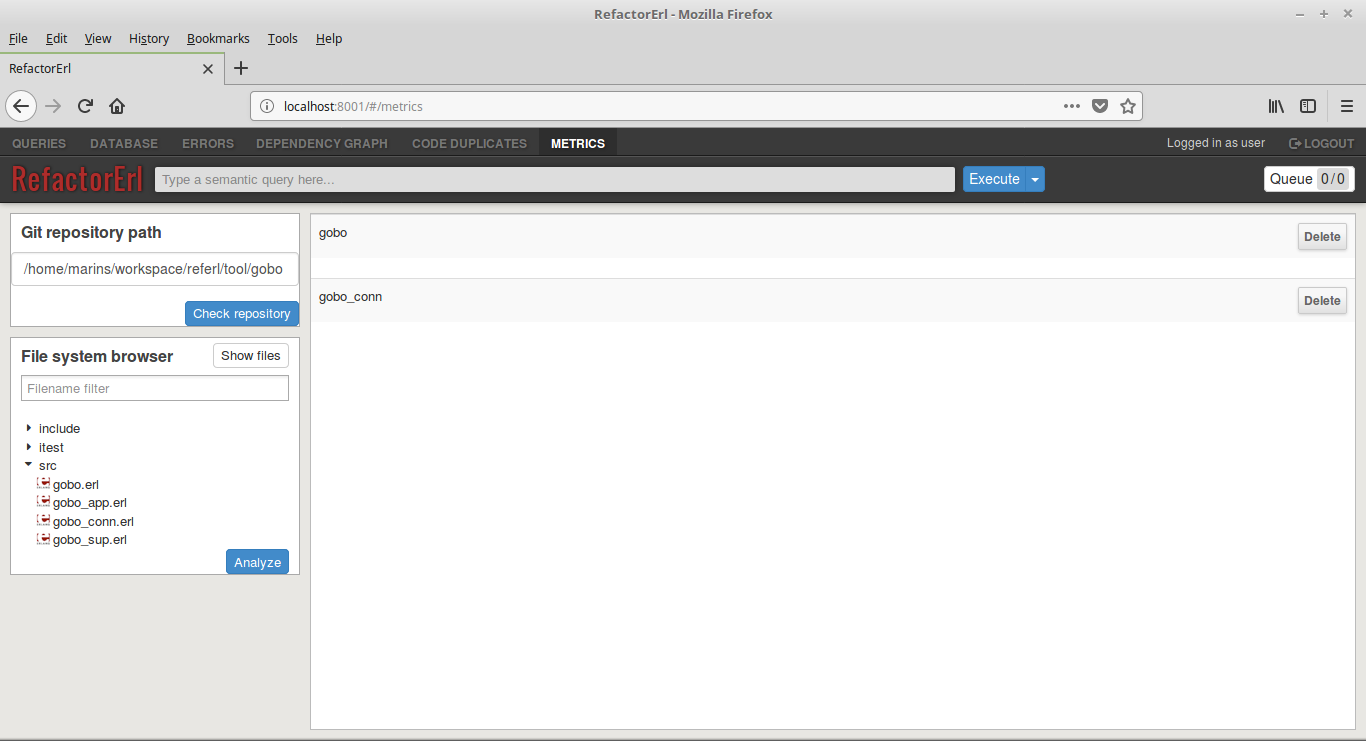
\includegraphics[height=80mm]{figures/files.png}
	\caption{Repository tree.}
	\label{fig:metrics_files}
\end{figure}

The final step is pressing "Analyze" button. It will start calculating metrics for all versions of the repository and progress will be shown on screen Figure \ref{fig:metrics_analyze}. 

\begin{figure}[h]
	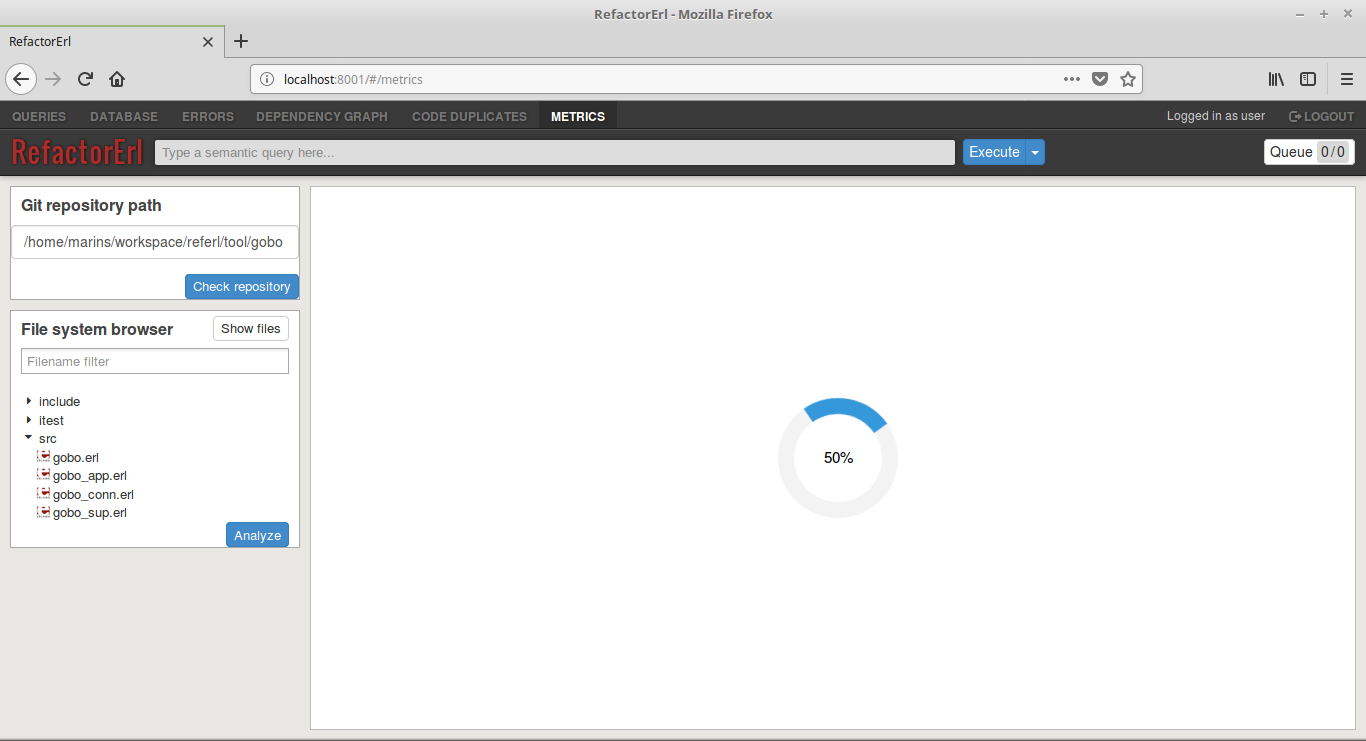
\includegraphics[height=80mm]{figures/analyze.png}
	\caption{The process of repository analyzing.}
	\label{fig:metrics_analyze}
\end{figure}

After analyzis is done the menu with choosing parameters of drawing the plot will be available as shown at Figure \ref{fig:metrics_plot}.

\begin{figure}[h]
	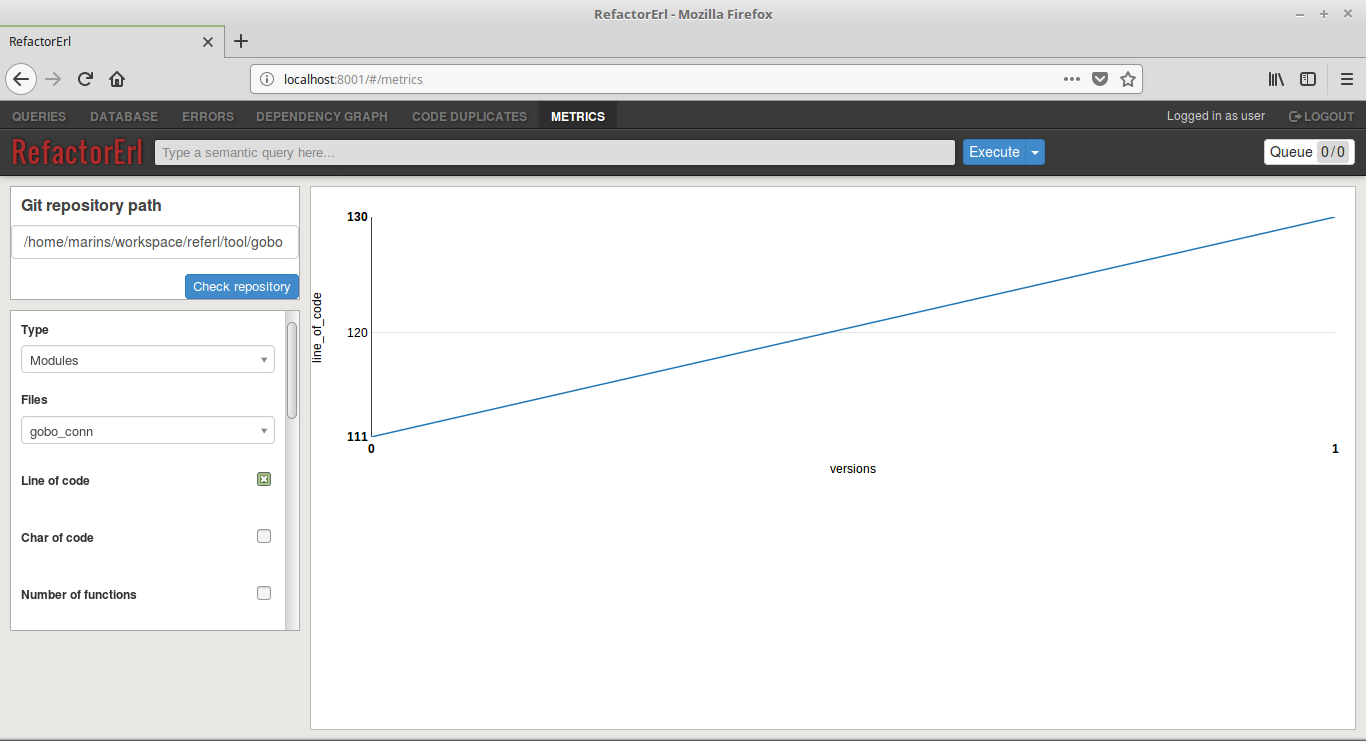
\includegraphics[height=80mm]{figures/plot.png}
	\caption{The example of plot.}
	\label{fig:metrics_plot}
\end{figure}